% Copyright (C) 2022 - Joseph Muré

\documentclass{beamer}

%\setbeameroption{hide notes}
%\setbeameroption{show notes}
%\setbeameroption{show only notes}

% Copyright (C) 2012 - EDF R&D - Michael Baudin

% To highlight source code
\usepackage{listings}
\definecolor{darkgreen}{rgb}{0,0.5,0}
\definecolor{violet}{rgb}{0.5,0,1}

\usepackage{lmodern}% http://ctan.org/pkg/lm

\usetheme{Montpellier}
\setbeamertemplate{navigation symbols}{} % Remove navigation
\useoutertheme{infolines}

\usepackage[utf8]{inputenc}
\usepackage[T1]{fontenc}

\usepackage{graphicx}
\unitlength=1cm
\graphicspath{{./figures/}}

\usepackage{hyperref}
\hypersetup{colorlinks=true, linkcolor=blue, linktocpage, urlcolor=blue}

\def\bx{{\bf x}}
\def\RR{\mathbb{R}}

\newcommand{\pyvar}[1]{\texttt{#1}}

\def \ot {OpenTURNS}

\definecolor{codegreen}{rgb}{0,0.6,0}
\definecolor{codegray}{rgb}{0.5,0.5,0.5}
\definecolor{codepurple}{rgb}{0.58,0,0.82}
\definecolor{backcolour}{rgb}{0.95,0.95,0.92}
\lstdefinestyle{mystyle}{
  backgroundcolor=\color{backcolour},   commentstyle=\color{codegreen},
  keywordstyle=\color{magenta},
  numberstyle=\tiny\color{codegray},
  stringstyle=\color{codepurple},
  basicstyle=\ttfamily\tiny,
  breakatwhitespace=false,         
  breaklines=true,                 
  captionpos=b,                    
  keepspaces=true,                 
  numbers=left,                    
  numbersep=5pt,                  
  showspaces=false,                
  showstringspaces=false,
  showtabs=false,                  
  tabsize=1,
  numbers=none
}

\lstset{style=mystyle, language=python}


\usepackage[
backend=biber,
style=alphabetic,
sorting=ynt
]{biblatex}

\usepackage{tikz}
\usetikzlibrary{positioning}

\renewcommand{\footnotesize}{\tiny}

\addbibresource{siamuq-2022-slides-OpenTURNS.bib}

\title[OpenTURNS]{Overview of OpenTURNS, its new features and its graphical user interface}

\author[Mur\'e et al.]{
J. Mur\'e \inst{1} \and
M. Baudin \inst{1} \and
J. Pelamatti \inst{1} \and
A. Dutfoy \inst{1} \and
O.~Mircescu \inst{1} \and
J. Schueller \inst{2} \and
T. Yalamas \inst{2}
}

\institute[EDF-Phim\'eca]{
\inst{1} EDF R\&D. 6, quai Watier, 78401, Chatou Cedex - France, joseph.mure@edf.fr \and %
\inst{2} Phimeca Engineering. 18/20 boulevard de Reuilly, 75012 Paris - France, yalamas@phimeca.com
}

\date[]{April 15th 2022, SIAM UQ 2022, Atlanta, US}

\definecolor{codegreen}{rgb}{0,0.6,0}
\definecolor{codegray}{rgb}{0.5,0.5,0.5}
\definecolor{codepurple}{rgb}{0.58,0,0.82}
\definecolor{backcolour}{rgb}{0.95,0.95,0.92}
\lstdefinestyle{mystyle}{
  backgroundcolor=\color{backcolour},   commentstyle=\color{codegreen},
  keywordstyle=\color{magenta},
  numberstyle=\tiny\color{codegray},
  stringstyle=\color{codepurple},
  basicstyle=\ttfamily\tiny,
  breakatwhitespace=false,         
  breaklines=true,                 
  captionpos=b,                    
  keepspaces=true,                 
  numbers=left,                    
  numbersep=5pt,                  
  showspaces=false,                
  showstringspaces=false,
  showtabs=false,                  
  tabsize=1,
  numbers=none
}

\lstset{style=mystyle, language=python}

%%%%%%%%%%%%%%%%%%%%%%%%%%%%%%%%%%%%%%%%%%%%%%%%%%%%%%%%%%%%%%%%%%%%%%%%%%%%%

  \begin{document}

%%%%%%%%%%%%%%%%%%%%%%%%%%%%%%%%%%%%%%%%%%%%%%%%%%%%%%%%%%%%%%%%%%%%%%%%%%%%%

  \begin{frame}
  \titlepage
  
  \begin{columns}
    \column{0.45\textwidth}
  \begin{center}

\includegraphics[height=0.15\textheight]{figures/edf.jpg}
\end{center}
    \column{0.1\textwidth}
	
    \column{0.45\textwidth}
  \begin{center}

\includegraphics[height=0.15\textheight]{figures/logo_phimeca.png}
\end{center}
  \end{columns}

  \end{frame}


%%%%%%%%%%%%%%%%%%%%%%%%%%%%%%%%%%%%%%%%%%%%%%%%%%%%%%%%%%%%%%%%%%%%%%%%%%%%%

% \begin{frame}
% \frametitle{Contents}
% \tableofcontents
% \end{frame}

%%%%%%%%%%%%%%%%%%%%%%%%%%%%%%%%%%%%%%%%%%%%%%%%%%%%%%%%%%%%%%%%%%%%%%%%%%%%%
\section{Introduction}

%%%%%%%%%%%%%%%%%%%%%%%%%%%%%%%%%%%%%%%%%%%%%%%%%%%%%%%%%%%%%%%%%%%%%%%%%%%%%

\begin{frame}
\frametitle{OpenTURNS: \url{www.openturns.org}}


    \begin{center}
    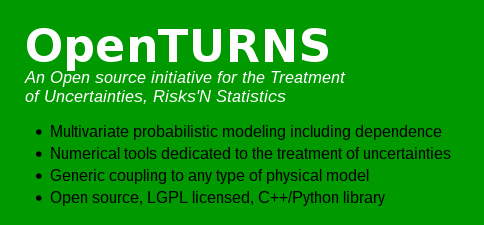
\includegraphics[width=0.8\textwidth]{figures/OT.png}
    \end{center}
	
\begin{itemize}
\item Multivariate probabilistic modeling including dependence
\item Numerical tools dedicated to the treatment of uncertainties
\item Generic coupling to any type of physical model
\item Open source, LGPL licensed, C++/Python library
\end{itemize}


\end{frame}

\note{
OpenTURNS is software for uncertainty quantification, uncertainty propagation,
sensitivity analysis and metamodeling. 

It is available with the open source LGPL licence on Linux, Windows and macOS.

In order to use OpenTURNS, you can use directly the C++ library, or 
program your Python scripts. 
}
%%%%%%%%%%%%%%%%%%%%%%%%%%%%%%%%%%%%%%%%%%%%%%%%%%%%%%%%%%%%%%%%%%%%%%%%%%%%%

\begin{frame}
\frametitle{OpenTURNS: \url{www.openturns.org}}

\begin{center}
   \begin{tabular}{ccccc}
   
\includegraphics[width=0.07\textwidth]{figures/logoEDF_Anne.png}&
   
\includegraphics[width=0.12\textwidth]{figures/LogoAirbus.png}&
   
\includegraphics[width=0.12\textwidth]{figures/logo_phimeca.png}&
   
\includegraphics[width=0.12\textwidth]{figures/logo_Imacs.png}
   
\includegraphics[width=0.30\textwidth]{figures/logo_ONERA.jpg}&
   \end{tabular}
\end{center}

\vspace*{0.05cm}
\begin{itemize}
\item Linux, Windows, macOS
\item First release : 2007
\item 5 full time developers
\item Users $\approx 1000$, mainly in France
(785 000 Total Conda downloads)
\item Project size : 800  classes, more than 6000 services
\end{itemize}


\end{frame}

%%%%%%%%%%%%%%%%%%%%%%%%%%%%%%%%%%%%%%%%%%%%%%%%%%%%%%%%%%%%%%%%%%%%%%%%%%%%%

\begin{frame}[containsverbatim]
  \frametitle{OpenTURNS: content}
  
  \begin{scriptsize}
  
  \begin{minipage}[t]{0.33\textwidth}
  \begin{itemize}
  \item Data analysis
  \begin{itemize}
  \tiny
  \item Distribution fitting
  \item Statistical tests
  \item Estimate dependency and copulas
  \item Estimate stochastic processes
  \end{itemize}
  \end{itemize}
  \end{minipage}%
  \begin{minipage}[t]{0.33\textwidth}
  \begin{itemize}
  \item Probabilistic modeling
  \begin{itemize}
  \tiny
  \item Dependence modeling
  \item Univariate distributions
  \item Multivariate distrbutions
  \item Copulas
  \item Processes 
  \item Covariance kernels
  \end{itemize}
  \end{itemize}
  \end{minipage}%
  \begin{minipage}[t]{0.33\textwidth}
  \begin{itemize}
  \item Surrogate models
  \begin{itemize}
  \tiny
  \item Linear regression
  \item Polynomial chaos expansion
  \item Gaussian  process regression
  \item Spectral methods
  \item Low rank tensors
  \item Fields metamodel
  \end{itemize}
  \end{itemize}
  \end{minipage}
  
  \vspace{20pt}  
  
  \begin{minipage}[t]{0.33\textwidth}
  \begin{itemize}
  \item Reliability, sensitivity
  \begin{itemize}
  \tiny
  \item Sampling methods
  \item Approximation methods
  \item Sensitivity analysis
  \item Design of experiments
  \end{itemize}
  \end{itemize}
  \end{minipage}%
  \begin{minipage}[t]{0.33\textwidth}
  \begin{itemize}
  \item Calibration
  \begin{itemize}
  \tiny
  \item Least squares calibration
  \item Gaussian calibration
  \item Bayesian calibration
  \end{itemize}
  \end{itemize}
  \end{minipage}%
  \begin{minipage}[t]{0.33\textwidth}
  \begin{itemize}
  \item Numerical methods
  \begin{itemize}
  \tiny
  \item Optimization
  \item Integration
  \item Least squares 
  \item Meshing
  \item Coupling with external codes
  \end{itemize}
  \end{itemize}
  \end{minipage}
  \end{scriptsize}

  \begin{tabular}{@{}c@{}c@{}c@{}c@{}c@{}}
  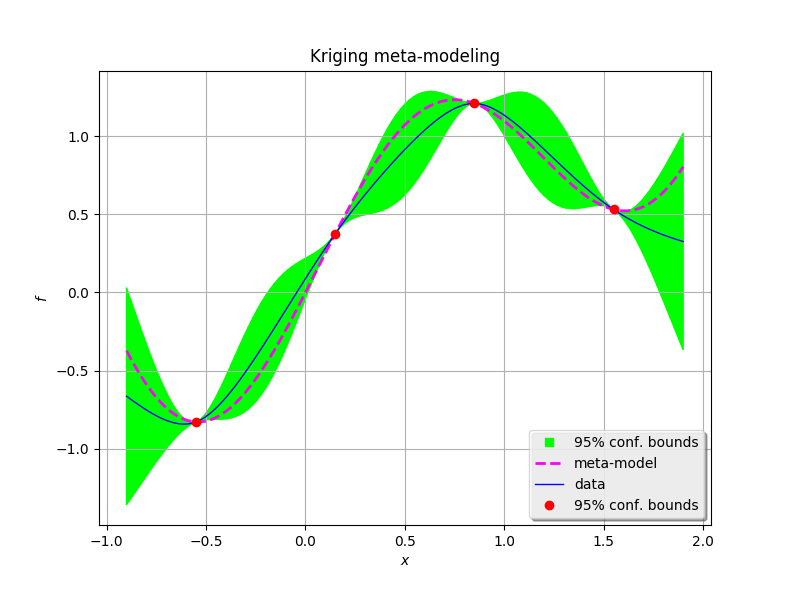
\includegraphics[width=0.2\textwidth]{figures/plot_kriging.png}&
  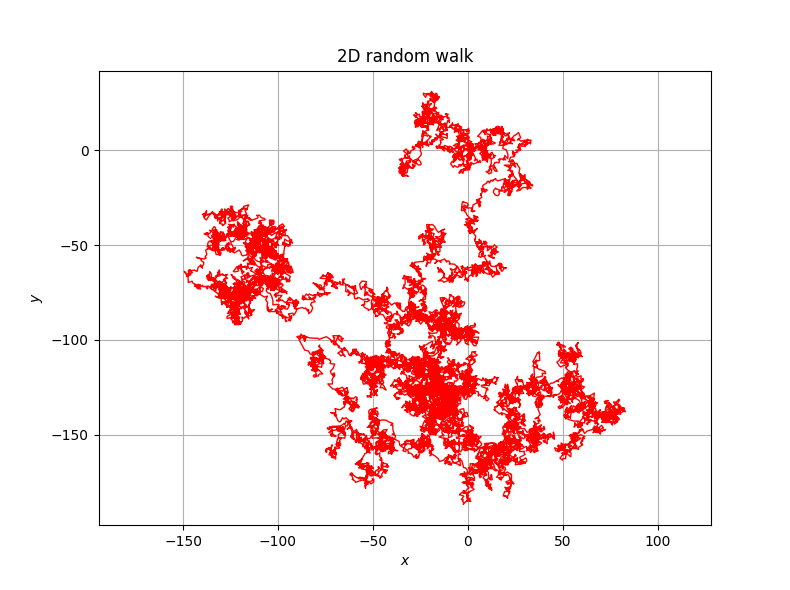
\includegraphics[width=0.2\textwidth]{figures/plot_random_walk.png}&
  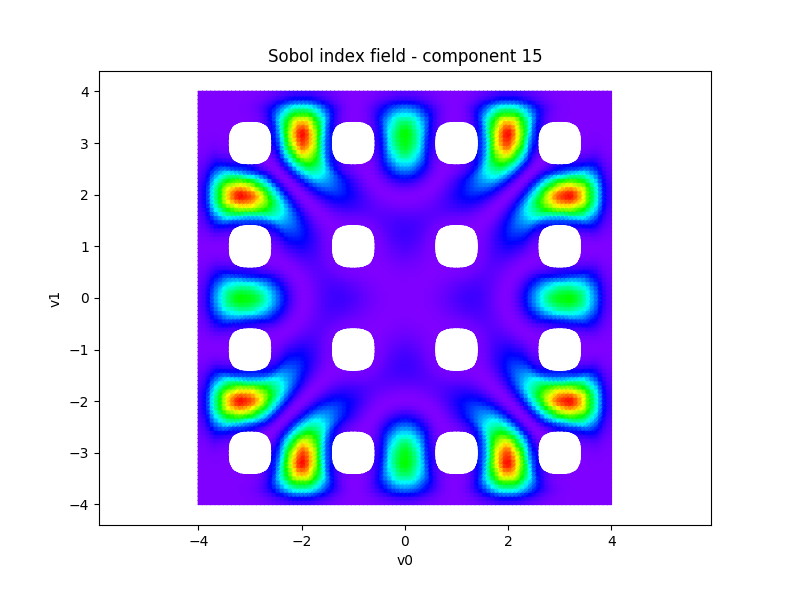
\includegraphics[width=0.2\textwidth]{figures/plot_sobol_field.png}&
  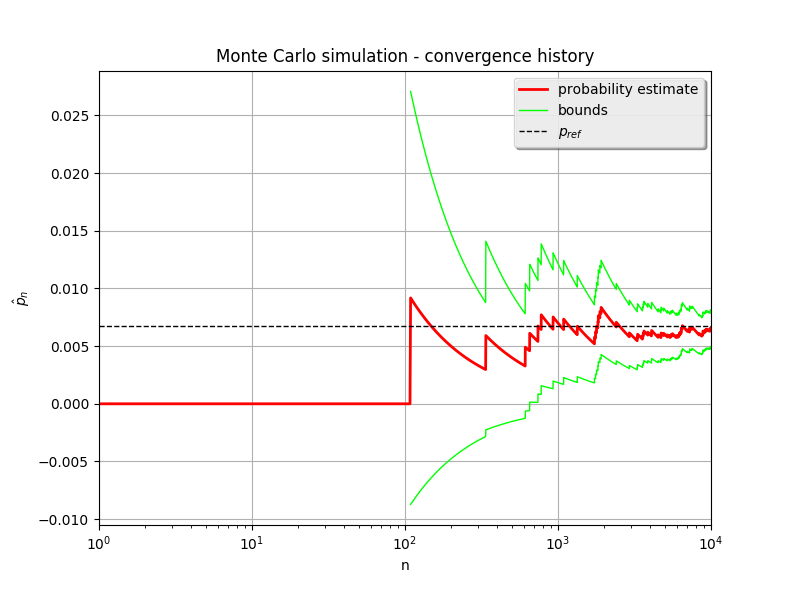
\includegraphics[width=0.2\textwidth]{figures/plot_monte_carlo.png}&
  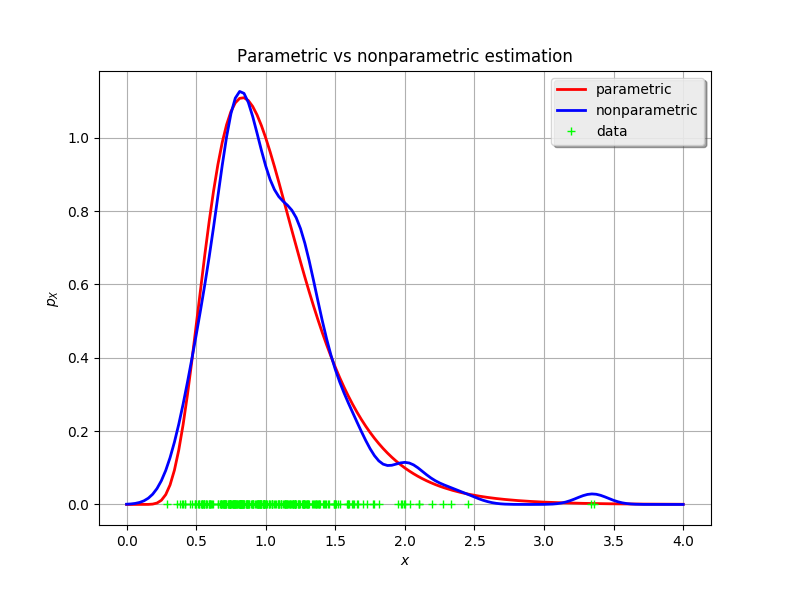
\includegraphics[width=0.2\textwidth]{figures/plot_distribution_fitting.png}
  \end{tabular}
\end{frame}
  
  
%%%%%%%%%%%%%%%%%%%%%%%%%%%%%%%%%%%%%%%%%%%%%%%%%%%%%%%%%%%%%%%%%%%%%%%%%%%%%

\begin{frame}[containsverbatim]
  \frametitle{OpenTURNS: documentation}
  
  \small{
  
  \begin{columns}
      \column{0.5\textwidth}
  
      \begin{center}
      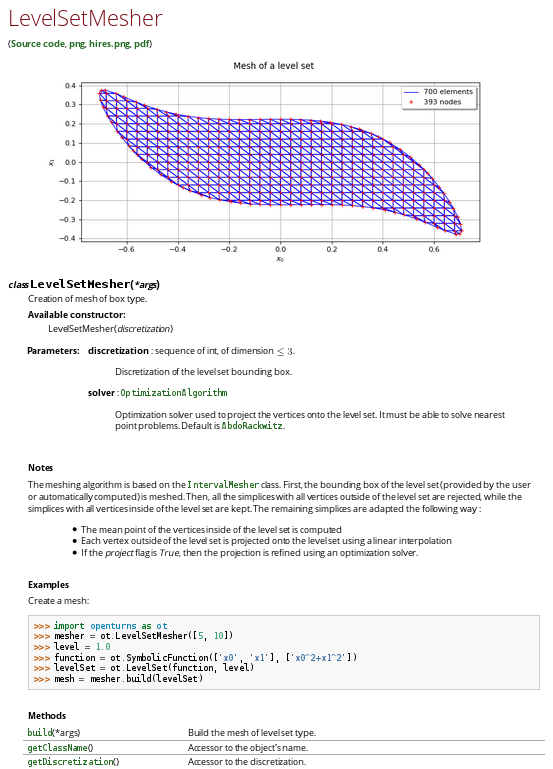
\includegraphics[width=0.8\textwidth]{figures/exClasses.png}
      \end{center}
  
      \column{0.5\textwidth}
  
    \begin{itemize}
    \item \underline{Content}: 
    \begin{itemize}
    \item Programming interface (API)
    \item Examples
    \item Theory
    \end{itemize}
    \item \emph{All} classes and methods 
    are documented, partly automatically.
    \item Examples are automatically tested at \emph{each} update 
    of the code and outputs are checked.
    \end{itemize}
    
  \end{columns}
  
  }
\end{frame}
  
%%%%%%%%%%%%%%%%%%%%%%%%%%%%%%%%%%%%%%%%%%%%%%%%%%%%%%%%%%%%%%%%%%%%%%%%%%%%%

\begin{frame}[containsverbatim]
  \frametitle{OpenTURNS: practical use}
  
  \small
  \begin{itemize}
  \item Compatibility with most popular python packages
  \begin{itemize}
  \scriptsize
  \item Numpy
  \item Scipy
  \item Matplotlib
  \item scikit-learn
  \end{itemize}
  \vspace{10pt}
  \item Parallel computational with shared memory (TBB)
  \vspace{10pt}
  \item Optimized linear algebra with LAPACK and BLAS 
  \vspace{10pt}
  \item Possibility to interface with a computation cluster
  \vspace{10pt}
  \item Focused towards handling numerical data
  \vspace{10pt}
  \item Installation through conda, pip, packages for various Linux distros and source code
  \end{itemize}
\end{frame}
  

%%%%%%%%%%%%%%%%%%%%%%%%%%%%%%%%%%%%%%%%%%%%%%%%%%%%%%%%%%%%%%%%%%%%%%%%%%%%%

\begin{frame}[containsverbatim]
  \frametitle{Coupling OpenTURNS with computer codes}
  
  \small
  
  OpenTURNS provides a text file exchange based interface in order to perform analyses on complex computer codes
  
  \vspace{10pt}
  
  \begin{columns}
      \column{0.6\textwidth}
      
  \centering
  
  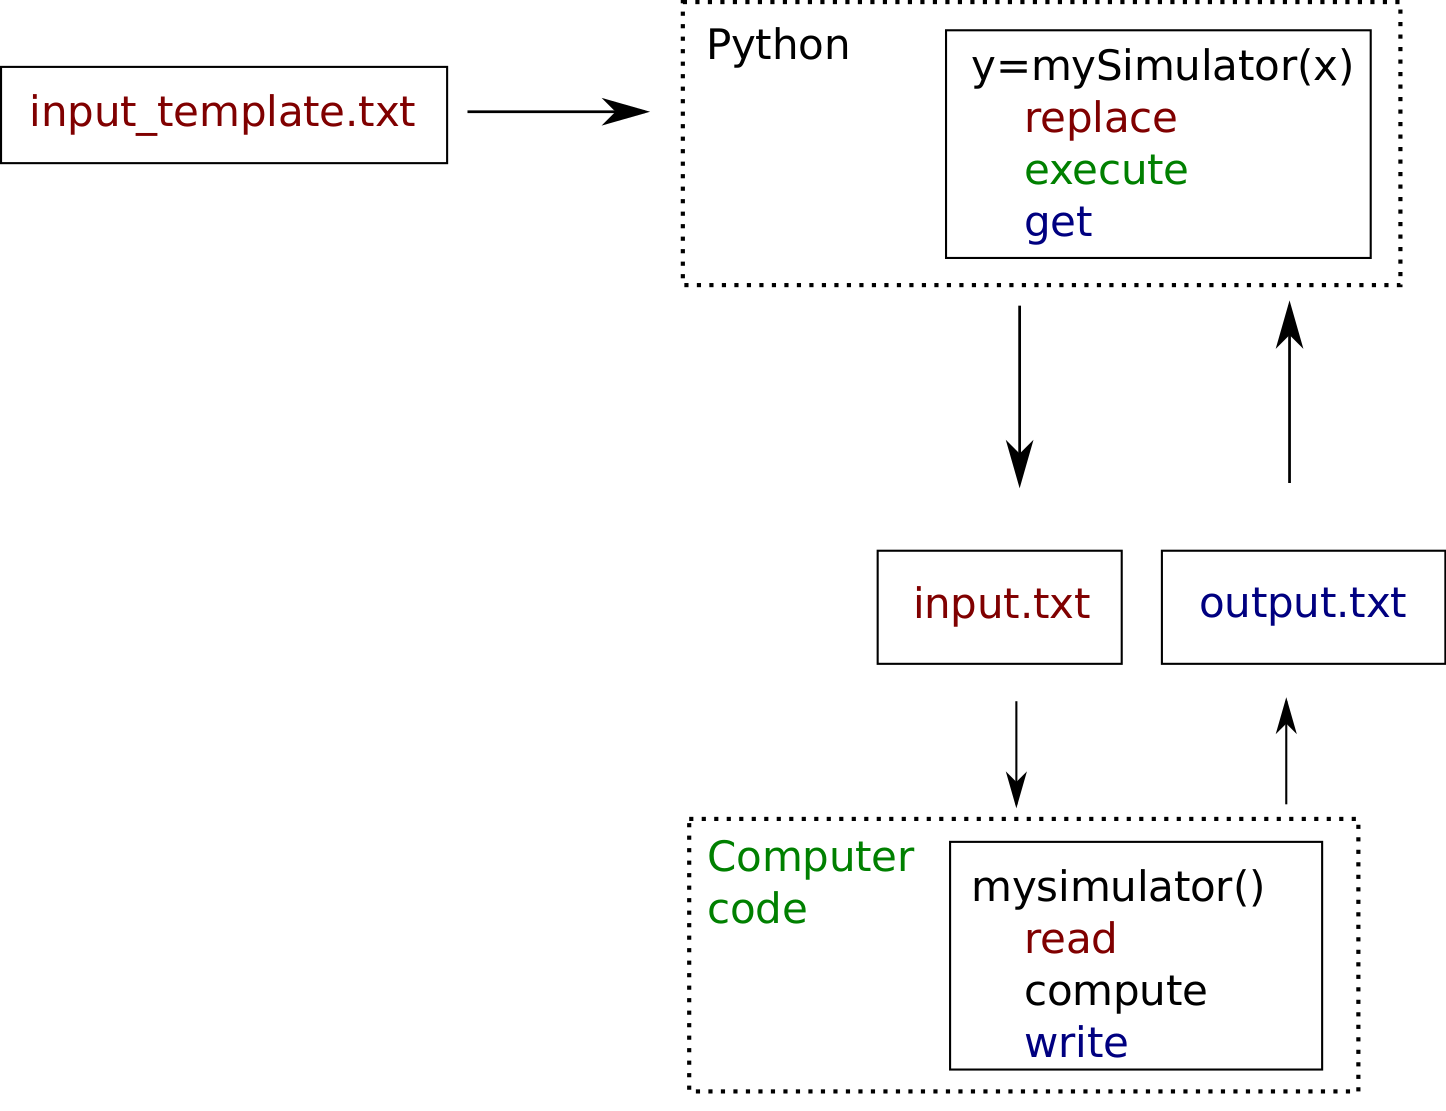
\includegraphics[width=1.\textwidth]{figures/Coupling.png}
  
      \column{0.4\textwidth}
  
  \begin{itemize}
  \item Replaces the need for input/output text parsers
  \item Wraps a simulation code under the form of a standard python function
  \item Allows to interface OpenTURNS with a cluster
  \item \href{https://openturns.github.io/otwrapy/master/index.html}{otwrapy}: interfacing tool to allow easy parallelization
  \end{itemize}
  
  \end{columns}
  
\end{frame}

%%%%%%%%%%%%%%%%%%%%%%%%%%%%%%%%%%%%%%%%%%%%%%%%%%%%%%%%%%%%%%%%%%%%%%%%%%%%%

\section{OpenTURNS 1.22: New capabilities}

%%%%%%%%%%%%%%%%%%%%%%%%%%%%%%%%%%%%%%%%%%%%%%%%%%%%%%%%%%%%%%%%%%%%%%%%%%%%%

\begin{frame}
  \frametitle{Functional surrogate model}
  
  \small
      \begin{itemize}
        \item We want a surrogate $\hat{h}$ of a model $h$ that maps a time series to a vector:
        \begin{equation*}
          h: \mathcal{F}([0, 1], \mathbb{R}^d) \rightarrow \mathbb{R}^p
        \end{equation*}
        % \begin{equation*}
        % \mathbf{X} = (X_1, X_2, \dots, X_d)^{\top} \sim P_{\mathbf{X}} \quad\mbox{over}\quad \mathcal{X} = \times_{i=1}^{d} \mathcal{X}_i
        % \end{equation*}
        % \vspace{-10pt}
        % \begin{equation*}
        % \mathcal{M} : \left|\begin{array}{rcl}
        % \mathcal{X} \subseteq \mathbb{R}^d & \longrightarrow & \mathcal{Y} \subseteq \mathbb{R}\\
        % \mathbf{X} & \longrightarrow & Y = \mathcal{M}(\mathbf{X})
        % \end{array}
        % \right.
        % \end{equation*}
        % \vspace{10pt}
        % \item \textbf{Learning sample} $\rightarrow$ a $n$-size i.i.d. sample of the couple $(\mathbf{X},Y)$:
        % \begin{equation*}
        % \left(\mathbf{X}^{(j)}, Y^{(j)}\right)_{(1\leq j\leq n)} = \left(X_1^{(j)}, X_2^{(j)}, \dots, X_d^{(j)}, Y^{(j)}\right)_{(1\leq j\leq n)}
        % \end{equation*}
        % with $P_{\mathbf{X}^{(j)}} = P_{\mathbf{X}}$ and $Y^{(j)} = \mathcal{M}\left(X_1^{(j)}, X_2^{(j)}, \dots, X_d^{(j)}\right)$, $\forall j \in \{1,\dots,n\}$
      \end{itemize}
  \vspace{-0.7cm}
  \begin{columns}
    \column{0.2\textwidth}
    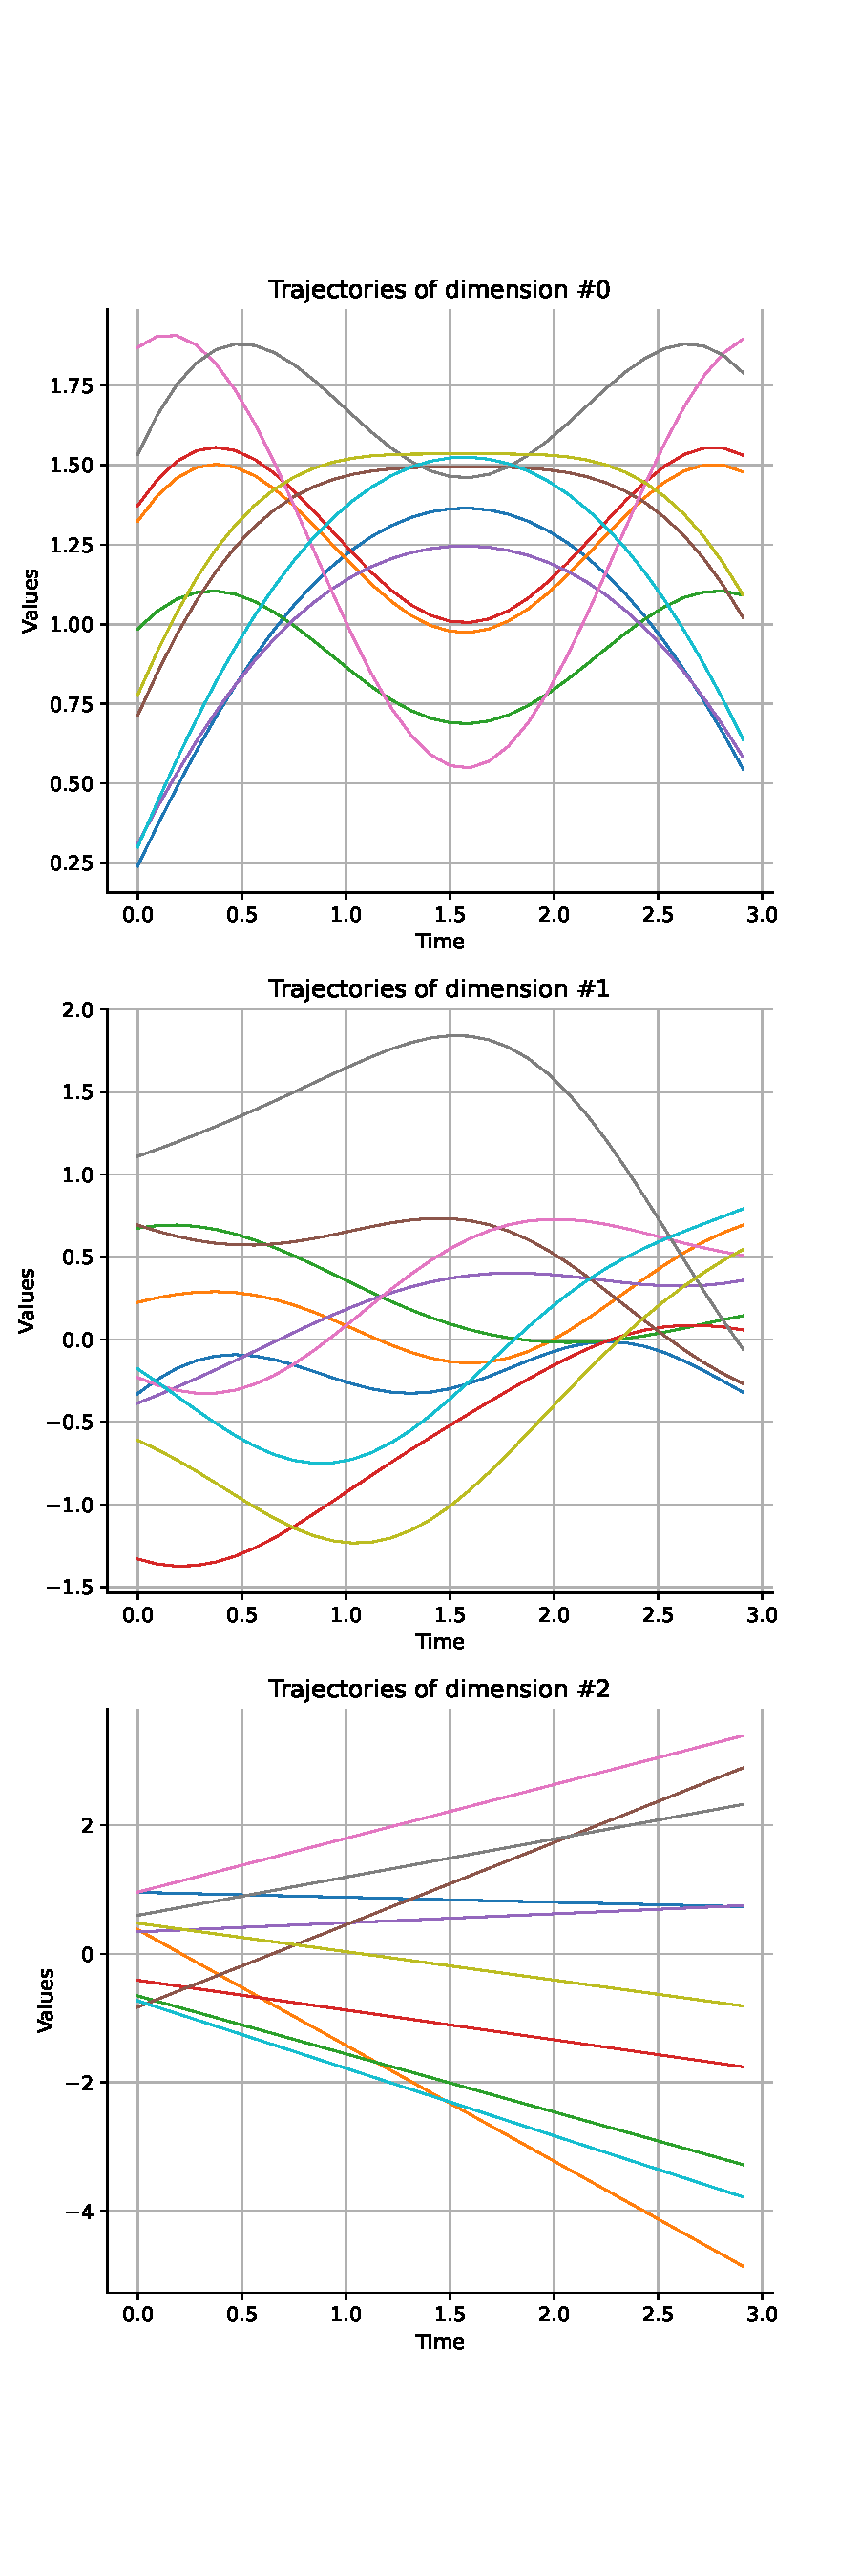
\includegraphics[width=.99\textwidth]{figures/time_series.pdf}
    \column{0.7\textwidth}
    \hspace{-0.5cm}
    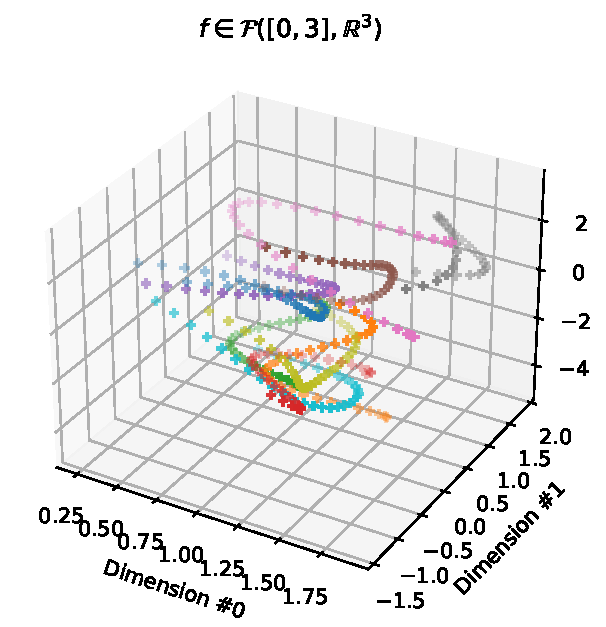
\includegraphics[width=.99\textwidth]{figures/scatter_3d.pdf}
    \column{0.1\textwidth}
    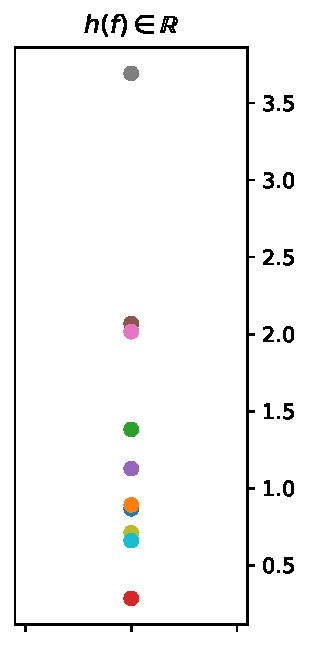
\includegraphics[width=.99\textwidth]{figures/response.pdf}
  \end{columns}

  \end{frame}

  
%%%%%%%%%%%%%%%%%%%%%%%%%%%%%%%%%%%%%%%%%%%%%%%%%%%%%%%%%%%%%%%%%%%%%%%%%%%%%%
  
  \begin{frame}[containsverbatim]
  \frametitle{Functional surrogate model: \texttt{FieldToPointFunctionalChaosAlgorithm}}
  
  \begin{itemize}
    \item We build the surrogate $\hat{h} : \mathcal{F}([0, 1], \mathbb{R}^d) \rightarrow \mathbb{R}^p$ from $N$ observations.
    \item Define the observations:
  \end{itemize}

    \begin{lstlisting}
    timegrid = ot.RegularGrid(start, step, N)
    collection = ... # collection of numpy arrays with shape (N, d)
    x = ot.ProcessSample(timegrid, collection) # functional input data
    y = ... # numpy array of shape (N, p)
    \end{lstlisting}
    
    \begin{itemize}
    \item Step 1: for each dimension of the input data, perform PCA.
    \item Step 2: build a polynomial chaos mappling the PCA coefficients to the outputs
    \item The \texttt{FieldToPointFunctionalChaosAlgorithm} experimental class does both steps at once:
    \end{itemize}

    \begin{lstlisting}
    from openturns.experimental import FieldToPointFunctionalChaosAlgorithm
    algo = FieldToPointFunctionalChaosAlgorithm(x, y)
    algo.setThreshold(0.04) # part of the variance unexplained by the PCA
    algo.run()
    result = algo.getResult()
    \end{lstlisting} 
  

  \end{frame}
  
  
  %%%%%%%%%%%%%%%%%%%%%%%%%%%%%%%%%%%%%%%%%%%%%%%%%%%%%%%%%%%%%%%%%%%%%%%%%%%%%
  
  \begin{frame}[containsverbatim]
  \frametitle{Functional surrogate model: validation (case where $p=1$)}
  
  \small
  \begin{lstlisting}
    x_valid = ... # input validation ProcessSample
    y_valid = ... # output values
    surrogate = result.getFieldToPointMetamodel() # h_hat
    yhat_valid = surrogate(x_valid)

    graph = ot.VisualTest.DrawQQplot(y_valid, yhat_valid) # graphical validation
    graph.setTitle("")
    graph.setXTitle("True output values")
    graph.setYTitle("Surrogate model values")
  \end{lstlisting} 

  \centering
  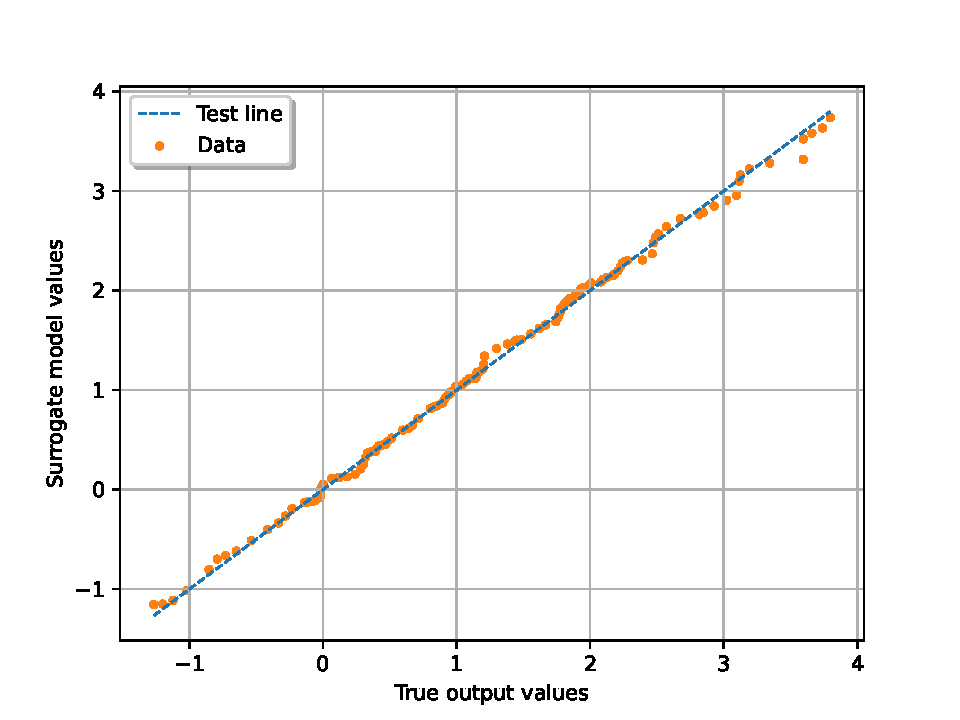
\includegraphics[width=.5\textwidth]{figures/validation.pdf}

  \end{frame}
  
%%%%%%%%%%%%%%%%%%%%%%%%%%%%%%%%%%%%%%%%%%%%%%%%%%%%%%%%%%%%%%%%%%%%%%%%%%%%%
  
\begin{frame}[containsverbatim]
\frametitle{Step 1 analysis: visualize and validate PCA modes}
\vspace{-0.3cm}
\begin{columns}
  \begin{column}{0.49\textwidth}
  \begin{lstlisting}
pca_l = result.getInputKLResultCollection()
grid = ot.GridLayout(1, d)
for num, pca in enumerate(pca_l):
    modes = pca.getModesAsProcessSample()
    graph = modes.drawMarginal(0)
    graph.setTitle(f"Dimension #{num}")
    grid.setGraph(0, num, graph)
  \end{lstlisting}    
  \end{column}
  \begin{column}{0.49\textwidth}
    \begin{lstlisting}
for num, pca in enumerate(pca_l):
    m = x.getMarginal(num)
    v = ot.KarhunenLoeveValidation(m, pca)
    graph= v.drawValidation().getGraph(0,0)
    ratio = 100.0 * pca.getSelectionRatio()
    graph.setTitle(f"Ratio = {ratio:.2f}%")
    grid.setGraph(0, num, graph)
    \end{lstlisting}    
    \end{column}  
\end{columns}

\vspace{-0.4cm}
\centering
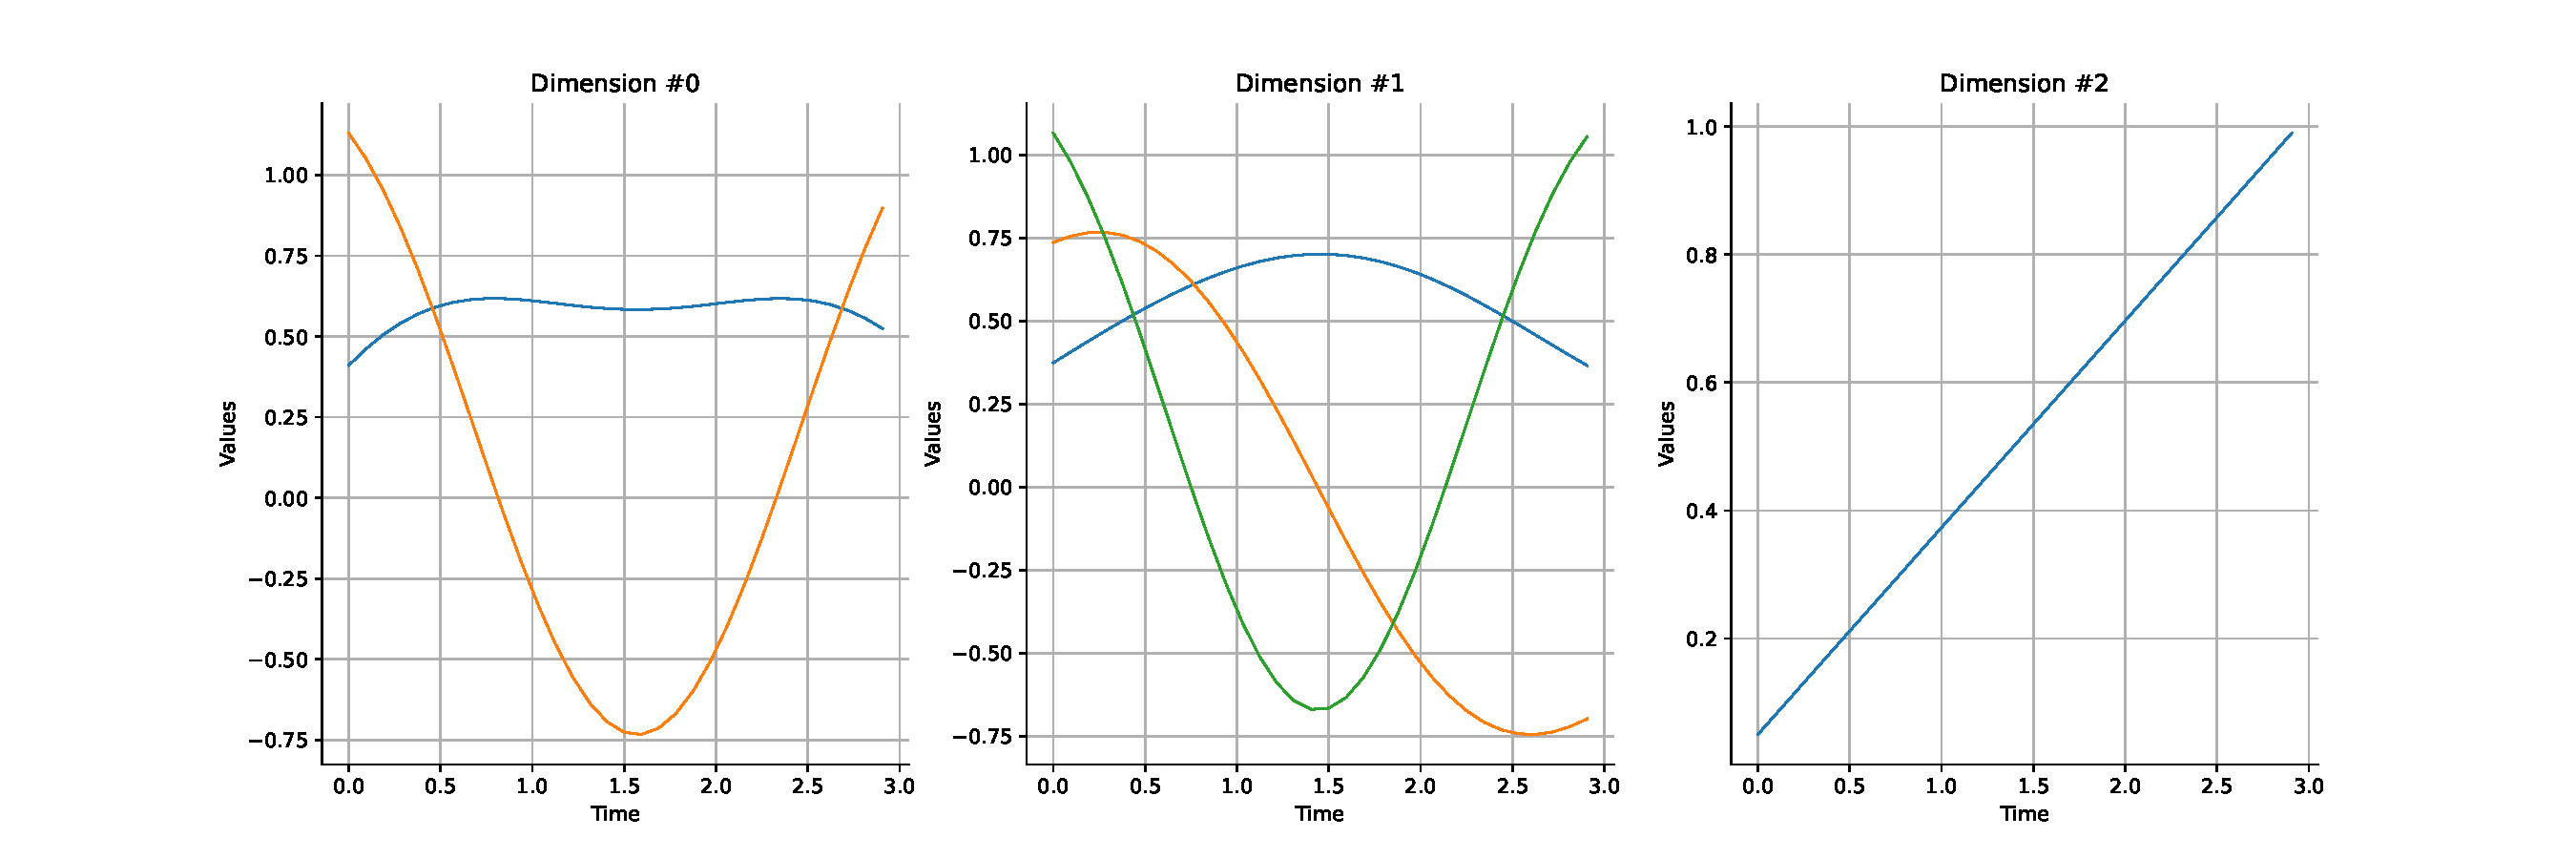
\includegraphics[width=0.8\textwidth]{figures/pca_modes.pdf}
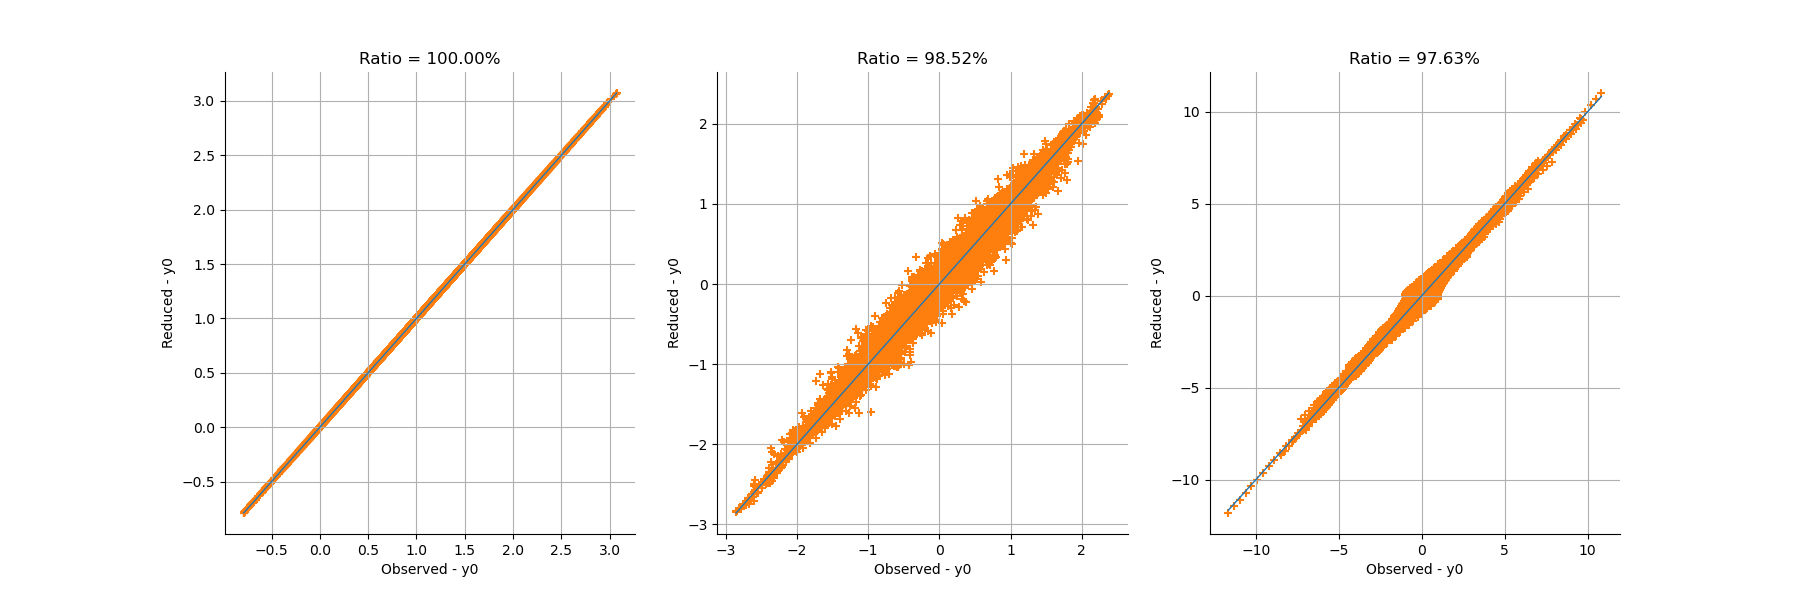
\includegraphics[width=0.8\textwidth]{figures/pca_validation.pdf}

\end{frame}
  
  
  
%%%%%%%%%%%%%%%%%%%%%%%%%%%%%%%%%%%%%%%%%%%%%%%%%%%%%%%%%%%%%%%%%%%%%%%%%%%%%
  
\begin{frame}[containsverbatim]
\frametitle{Step 2 analysis: polynomial-chaos-derived Sobol' indices}

\begin{lstlisting}
frop openturns.experimental import FieldFunctionalChaosSobolIndices
sensitivity = FieldFunctionalChaosSobolIndices(result)
graph = sensitivity.draw()
\end{lstlisting}

\centering
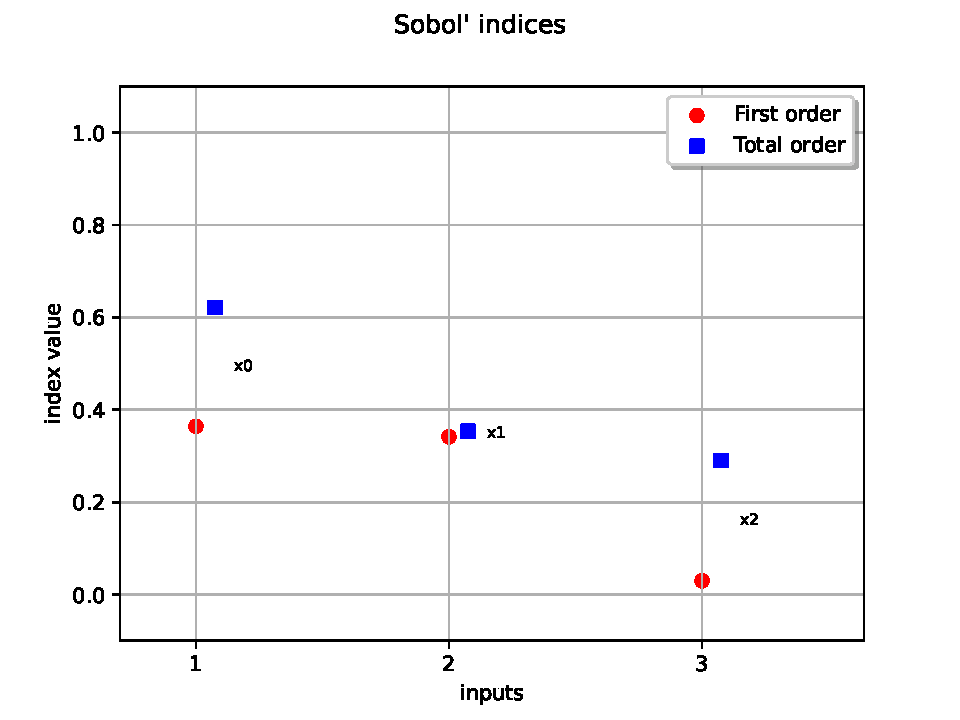
\includegraphics[width=0.7\textwidth]{figures/sobol.pdf}

\end{frame}
  
%%%%%%%%%%%%%%%%%%%%%%%%%%%%%%%%%%%%%%%%%%%%%%%%%%%%%%%%%%%%%%%%%%%%%%%%%%%%%

\begin{frame}[containsverbatim]
\frametitle{OpenTURNS: Metropolis-Hastings}
\small
We want to sample from the joint distribution $\pi$ of 3 random variables $X, Y, Z$.
Here is one step of the algorithm, starting from the point $(x, y, z)$:

\begin{enumerate}
\item Simulate a candidate $(x',y',z') \sim q( \cdot | x, y, z)$ for some conditional distribution $q$.
\item Compute
$
\alpha(x',y',z' | x,y,z) = \min \left\{ \frac{\pi(x',y',z') \, q(x,y,z | x',y',z')}{\pi(x,y,z) q(x',y',z' | x,y,z)} , 1 \right\}.
$
\item Simulate $u \sim \mathcal{U}(0,1)$. If $u \leqslant \alpha(x',y',z' | x,y,z)$,
then the next state is $(x',y',z')$, otherwise it is $(x,y,z)$.
\end{enumerate}

\begin{block}{Random walk Metropolis-Hastings}

When $q(\cdot | x, y, z) = (x,y,z) + \mu$, where $\mu$ is a distribution that does not depend on $(x,y,z)$,
the  algorithm is called ``Random walk Metropolis-Hastings'' and $\mu$ is called the ``proposal distribution''.

\begin{lstlisting}
init = [x_start, y_start, z_start]
proposal = ot.Normal(3) # steps follow a 3d normal distribution
mh = ot.RandomWalkMetropolisHastings(logdensity, support, init, proposal)
sample = mh.getSample(1000)
\end{lstlisting}
\end{block}

\end{frame}

\begin{frame}[containsverbatim]
\frametitle{OpenTURNS: Metropolis-Hastings variants}
\centering

\begin{block}{Single component randomwalk Metropolis-Hastings}
\medskip
\centering

\begin{tikzpicture}[
squarednode/.style={rectangle, draw=green!60, fill=green!5, very thick, minimum size=5mm},
]
%Nodes
\node[squarednode]      (mhx)                              {\texttt{mh\_x}};
\node[squarednode]      (mhy)       [right=of mhx] {{\texttt{mh\_y}}};
\node[squarednode]      (mhz)       [right=of mhy] {{\texttt{mh\_z}}};

%Lines
\draw[->] (mhx.east) -- (mhy.west);
\draw[->] (mhy.east) -- (mhz.west);
\draw[->] (mhz.east) to [out=340,in=200,looseness=1] (mhx.west);
\end{tikzpicture}

\begin{lstlisting}
prop_dim1 = ot.Normal(1) # steps follow a 1d normal distribution along one axis
mh_x = ot.RandomWalkMetropolisHastings(logdensity, support, init, prop_dim1, [0])
mh_y = ot.RandomWalkMetropolisHastings(logdensity, support, init, prop_dim1, [1])
mh_z = ot.RandomWalkMetropolisHastings(logdensity, support, init, prop_dim1, [2])
sample = ot.Gibbs([mh_x, mh_y, mh_z]).getSample(1000)
\end{lstlisting}

\end{block}

\begin{block}{Blocks of components can be considered}
\medskip
\centering

\begin{tikzpicture}[
squarednode/.style={rectangle, draw=green!60, fill=green!5, very thick, minimum size=5mm},
]
%Nodes
\node[squarednode]      (mhxy)                     {\texttt{mh\_xy}};
\node[squarednode]      (mhz)       [right=of mhxy] {\texttt{mh\_z}};

%Lines
\draw[->] (mhxy.east) -- (mhz.west);
\draw[->] (mhz.east) to [out=340,in=200,looseness=1.5] (mhxy.west);

\end{tikzpicture}

\begin{lstlisting}
prop_xy = ot.Normal(2) # steps follows a 2d normal distribution for (X,Y)
prop_z = ot.Normal(1)  # steps follow  a 1d normal distribution for Z
mh_xy = ot.RandomWalkMetropolisHastings(logdensity, support, init, prop_xy, [0, 1])
mh_z = ot.RandomWalkMetropolisHastings(logdensity, support, init, proposal, [2])
sample = ot.Gibbs([mh_xy, mh_z]).getSample(1000)
\end{lstlisting}  

\end{block}
\end{frame}


%%%%%%%%%%%%%%%%%%%%%%%%%%%%%%%%%%%%%%%%%%%%%%%%%%%%%%%%%%%%%%%%%%%%%%%%%%%%%

\begin{frame}[containsverbatim]
\frametitle{OpenTURNS: conditional samplers in Gibbs algorithms}
\small
Assume we have a direct sampler for $Z$ conditionally on $X$ and $Y$:
this sampler should be passed to the \texttt{RandomVectorMetropolisHastings} class.

\begin{lstlisting}
  z_sampler = ot.RandomVector(...) # build a direct sampler for Z | X, Y
  # Typically, Z depends on a function of (X,Y)
  # Write it as a function of (X,Y,Z) for the sake of genericity:
  f = ot.Function(...) # function f(X,Y,Z) which outputs the parameters of z_sampler
  mh_z = ot.RandomVectorMetropolisHastings(z_sampler, init, [2], f)

  prop_xy = ot.Normal(2) # steps follows a 2d normal distribution for (X,Y)
  mh_xy = ot.RandomWalkMetropolisHastings(logdensity, support, init, prop_xy, [0, 1])

  sample = ot.Gibbs([mh_x, mh_y, mh_z]).getSample(1000)
\end{lstlisting}
\centering
\includegraphics[width=.33\textwidth]{figures/gibbs_1.png}
\includegraphics[width=.66\textwidth]{figures/gibbs_2.png}

\end{frame}

%%%%%%%%%%%%%%%%%%%%%%%%%%%%%%%%%%%%%%%%%%%%%%%%%%%%%%%%%%%%%%%%%%%%%%%%%%%%%

\begin{frame}[containsverbatim]
  \frametitle{OpenTURNS: iterative statistics \footfullcite{pebay2008}  \footfullcite{meng2015}}
\small
\begin{columns}

  \column{0.54\textwidth}


  \begin{block}{Iterative moment estimation}
  \begin{lstlisting}
  iterMoments = ot.IterativeMoments(order, dim)

  # Iteratively compute the mean
  size = 2000
  meanEvolution = ot.Sample()
  for i in range(size):
      point = distNormal.getRealization()
      iterMoments.increment(point)
      meanEvolution.add(iterMoments.getMean())

  # Display the evolution
  ran = range(1, size + 1)
  iter_sample = ot.Sample.BuildFromPoint(ran)
  curve = ot.Curve(iter_sample, meanEvolution)
  graph = ot.Graph("Evolution of the mean",
                    "iteration nb",
                    "mean",
                    True)
  graph.add(curve)
  graph.setLogScale(ot.GraphImplementation.LOGX)
  view = otv.View(graph)
  \end{lstlisting}
  \end{block}

  \column{0.44\textwidth}

  \includegraphics[width=\textwidth]{figures/iter_mean.png}

  \begin{block}{Other available iterative stats}
    \begin{itemize}
      \item Extrema
      \item Threshold exceedance probability
    \end{itemize}
  \end{block}

\end{columns}

\end{frame}

%%%%%%%%%%%%%%%%%%%%%%%%%%%%%%%%%%%%%%%%%%%%%%%%%%%%%%%%%%%%%%%%%%%%%%%%%%%%%

\section{PERSALYS, the graphical user interface}

\begin{frame}
\frametitle{PERSALYS, the graphical user interface of \ot{}}
	
\begin{columns}
\column{0.7\textwidth}
	
\begin{itemize}
\item Provide a graphical interface of 
\ot{} in and out of the SALOME integration platform
\item Features : probabilistic model, 
	distribution fitting, central tendency, 
  sensitivity analysis, probability estimate, 
	surrogate modeling (polynomial chaos, kriging), screening (Morris), 
	optimization, design of experiments
\item GUI language : English, French

\item Partners : EDF, Phim\'eca
\item Licence : LGPL

\item Schedule : Since summer 2016, two releases per year, currently V12
\item On the internet (free) : SALOME\_EDF since 2018 on 
\url{www.salome-platform.org}

\end{itemize}

\column{0.3\textwidth}

\begin{center}

\includegraphics[width=0.95\textwidth]{figures/PERSALYS-LOGO.png}
\end{center}

\end{columns}


\end{frame}


%%%%%%%%%%%%%%%%%%%%%%%%%%%%%%%%%%%%%%%%%%%%%%%%%%%%%%%%%%%%%%%%%%%%%%%%%%%%%

\begin{frame}
\frametitle{Calibration}

Given a physical model $h$, observed inputs $\boldsymbol{x}$, 
observed outputs $y$ we can calibrate $\boldsymbol{\theta}$ so that 
$$
y = h(\boldsymbol{x}, \boldsymbol{\theta}) + \epsilon
$$
where $\epsilon$ is a random (Gaussian) variable.

Calibration outputs:
\begin{itemize}
\item the optimal value estimator $\hat{\boldsymbol{\theta}}$,
\item the distribution of $\hat{\boldsymbol{\theta}}$ and a confidence or credibility 
interval of each marginal,
\item the distribution of the residuals $\epsilon = y - h(\boldsymbol{x}, \hat{\boldsymbol{\theta}})$.
\end{itemize}

We implemented 4 methods\footnote{M. Baudin \& R. Lebrun, Linear algebra of linear and nonlinear Bayesian calibration. UNCECOMP 2021.} :

\begin{center}
\begin{tabular}{lll}
                     & {\bf Linear} & {\bf Non Linear} \\
\hline
No prior             & Least squares & Least squares \\
                     & linear        &  non linear \\
\hline
Gaussian prior       & Linear calib. & 3DVAR \\
\hline
\end{tabular}
\end{center}

\end{frame}


%%%%%%%%%%%%%%%%%%%%%%%%%%%%%%%%%%%%%%%%%%%%%%%%%%%%%%%%%%%%%%%%%%%%%%%%%%%%%

\begin{frame}
\frametitle{Calibration}

In PERSALYS, this requires:
\begin{itemize}
\item a physical model $h$ with parameters to calibrate, 
\item a data file containing the observed inputs and outputs.
\end{itemize}

\begin{center}
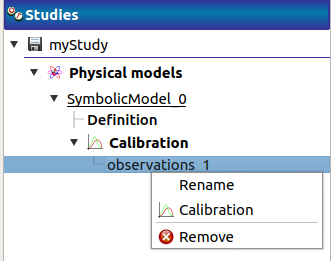
\includegraphics[width=0.35\textwidth]{figures/calibration_observations_contextMenu.png}
\end{center}

\begin{columns}
  \column{0.5\textwidth}

On output, we present the optimal value of each calibrated parameter, 
along with a 95\% confidence interval.

\column{0.5\textwidth}

\begin{center}
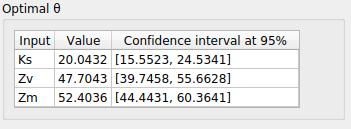
\includegraphics[width=0.9\textwidth]{figures/calibration-ks-zv-zm-optimal_focus.png}
\end{center}

\end{columns}
\end{frame}

%%%%%%%%%%%%%%%%%%%%%%%%%%%%%%%%%%%%%%%%%%%%%%%%%%%%%%%%%%%%%%%%%%%%%%%%%%%%%

\begin{frame}
  \frametitle{Calibration}
    
  \begin{center}
  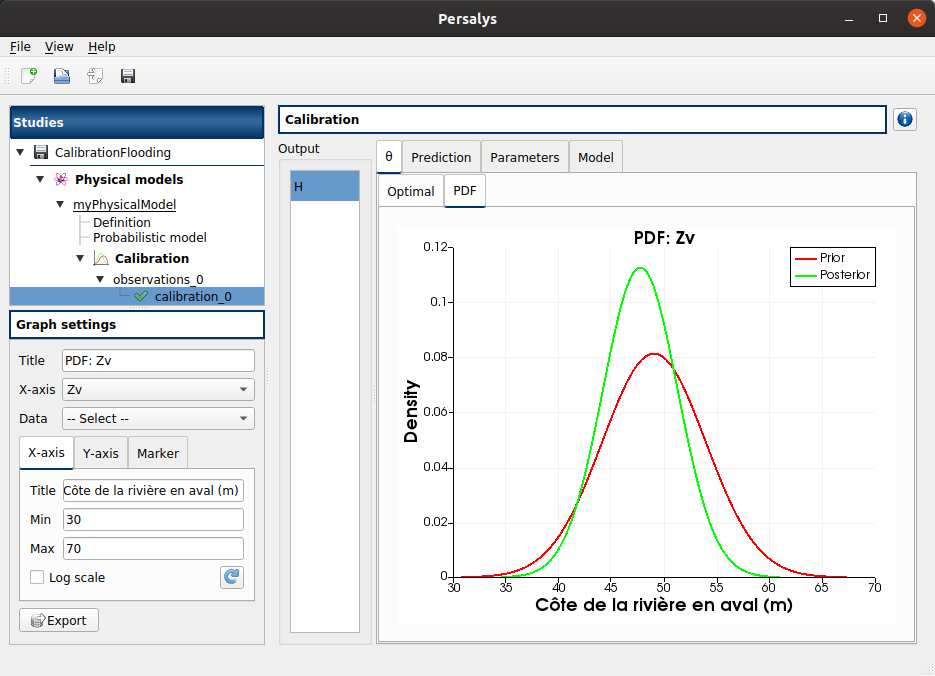
\includegraphics[width=0.86\textwidth]{figures/calibration-Zv-prior-posterior.png}
  \end{center}
  
  \end{frame}

%%%%%%%%%%%%%%%%%%%%%%%%%%%%%%%%%%%%%%%%%%%%%%%%%%%%%%%%%%%%%%%%%%%%%%%%%%%%%

\begin{frame}
\frametitle{What's next ?}
  \begin{columns}
    \column{0.5\textwidth}

PERSALYS Roadmap : 
\begin{itemize}
\item New surrogate models
\item 2D Fields, 3D Fields
\item In-Situ fields based on the MELISSA library (with INRIA): 
when we cannot store the whole sample in memory or on the hard drive, 
update the statistics (e.g. the mean, Sobol' indices) sequentially, 
with distributed computing. 
\end{itemize}

    \column{0.5\textwidth}

\begin{center}
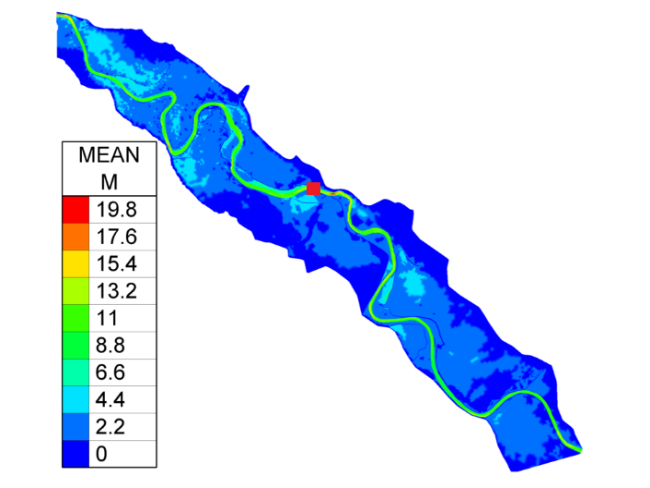
\includegraphics[height=0.5\textheight]{figures/image034.png}
\end{center}

	\end{columns}

\end{frame}

\note{

The next features we plan to add to PERSALYS is the management
of 2D and 3D stochastic fields. 

We also work on the use of the MELISSA software which performs 
in-situ studies. 

This library allows to perform UQ studies in situations 
where we cannot store more than a couple of multidimensional fields 
in memory or on the hard drive. 
}

%%%%%%%%%%%%%%%%%%%%%%%%%%%%%%%%%%%%%%%%%%%%%%%%%%%%%%%%%%%%%%%%%%%%%%%%%%%%%

\begin{frame}
\frametitle{The end}

\begin{center}
Thanks !
\end{center}

\begin{center}
Questions ?
\end{center}

\begin{columns}
\column{0.5\textwidth}
\centering

\includegraphics[width=0.5\textwidth]{figures/logo-openturns.png}
\column{0.5\textwidth}


\includegraphics[width=0.8\textwidth]{figures/PERSALYS-LOGO.png}

\end{columns}

\end{frame}
  
\end{document}
